% NLP Patient Description to Acuity — Deep-dive Beamer deck (~30 slides)
% Compile: pdflatex nlp_patient_to_acuity.tex && pdflatex nlp_patient_to_acuity.tex

\documentclass[10pt,aspectratio=169]{beamer}

\usetheme{AnnArbor}
\usecolortheme{spruce}
\setbeamercolor{title}{bg=green!60!black,fg=white}
\setbeamercolor{frametitle}{bg=green!60!black,fg=white}
\setbeamercolor{structure}{fg=green!60!black}
\setbeamercolor{palette primary}{bg=green!60!black,fg=white}
\setbeamercolor{palette secondary}{bg=green!70!black,fg=white}
\setbeamercolor{palette tertiary}{bg=green!80!black,fg=white}
\setbeamercolor{palette quaternary}{bg=black,fg=white}
\setbeamercolor{item}{fg=green!60!black}

\usepackage[T1]{fontenc}
\usepackage[utf8]{inputenc}
\usepackage{lmodern}
\usepackage{amsmath,amssymb}
\usepackage{booktabs}
\usepackage{array}
\usepackage{graphicx}
\usepackage{tikz}
\usetikzlibrary{positioning, arrows.meta, shapes.geometric, calc, fit}

\setbeamertemplate{navigation symbols}{}
\setbeamertemplate{footline}{%
	\hfill\small \insertframenumber{} / \inserttotalframenumber\hspace{1.5em}%
}

\definecolor{triageRed}{RGB}{220,20,60}
\definecolor{triageOrange}{RGB}{255,140,0}
\definecolor{triageYellow}{RGB}{255,200,0}
\definecolor{triageGreen}{RGB}{34,139,34}
\definecolor{triageBlue}{RGB}{30,64,175}

\tikzset{
	flowbox/.style={rectangle, draw=green!60!black, rounded corners=3pt,
		fill=green!6, minimum height=0.75cm, minimum width=1.6cm,
		align=center, font=\scriptsize, inner sep=3pt},
	flowarr/.style={-{Stealth[length=2mm]}, thick, draw=green!70!black},
	edgelabel/.style={font=\tiny, fill=white, inner sep=1pt},
	vartable/.style={font=\scriptsize}
}

\newcommand{\plain}[1]{\begin{block}{In plain English}\footnotesize #1\end{block}}
\newcommand{\complaint}{\textit{``I have a headache and feel feverish. My body aches and I feel weak.''}}

\title[NLP to Acuity]{NLP Patient Description to Acuity}
\subtitle{Deep Learning and Mathematical Triage}
\author{Quaigraine Samuel \and Twum Samuel}
\institute{Department of Mathematics\\Kwame Nkrumah University of Science and Technology}
\date{\today}

\begin{document}

\begin{frame}
	\titlepage
\end{frame}

\begin{frame}{Outline}
	\tableofcontents
\end{frame}

% =============================================================================
\section{Clinical Context}
% =============================================================================

\begin{frame}{The Clinical Scenario}
	\begin{columns}[T]
		\begin{column}{0.52\textwidth}
			\begin{center}
				
\includegraphics[width=\textwidth, height=0.34\textheight, keepaspectratio]{convo}
			\end{center}
			\vspace{0.1cm}
			\centering\scriptsize
			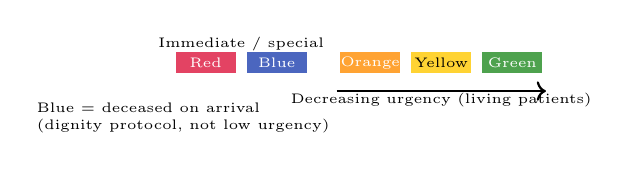
\begin{tikzpicture}[x=0.95cm]
				% Immediate / special protocols
				\fill[triageRed!80] (0,0.35) rectangle ++(0.8,0.26);
				\node[font=\tiny, white] at (0.4,0.48) {Red};
				\fill[triageBlue!80] (0.95,0.35) rectangle ++(0.8,0.26);
				\node[font=\tiny, white] at (1.35,0.48) {Blue};
				\node[font=\tiny, align=center] at (0.875,0.72) {Immediate / special};
				% Living-patient urgency scale
				\fill[triageOrange!80] (2.2,0.35) rectangle ++(0.8,0.26);
				\node[font=\tiny, white] at (2.6,0.48) {Orange};
				\fill[triageYellow!80] (3.15,0.35) rectangle ++(0.8,0.26);
				\node[font=\tiny, black] at (3.55,0.48) {Yellow};
				\fill[triageGreen!80] (4.1,0.35) rectangle ++(0.8,0.26);
				\node[font=\tiny, white] at (4.5,0.48) {Green};
				% Arrow below bars only (Orange -> Green)
				\draw[->, thick] (2.15,0.12) -- (4.95,0.12);
				\node[font=\tiny] at (3.55,0.0) {Decreasing urgency (living patients)};
				\node[font=\tiny, align=left] at (0.1,-0.22) {Blue = deceased on arrival\\(dignity protocol, not low urgency)};
			\end{tikzpicture}
		\end{column}
		\begin{column}{0.46\textwidth}
			\small
			\textbf{Setting:} Komfo Anokye Teaching Hospital (KATH), Kumasi --- \textbf{SATS} triage.

			\vspace{0.2cm}
			\textbf{Chief complaint (running example):}\\
			\complaint

			\vspace{0.2cm}
			How does a computer mathematically interpret this simple, unstructured complaint and convert it into a triage colour?

			\vspace{0.15cm}
			\footnotesize\textit{The system supports triage staff; it does not diagnose disease or replace clinical judgment.}
		\end{column}
	\end{columns}
\end{frame}

\begin{frame}{The Dual Pathway: TEWS vs.\ NLP Chatbot}
	\begin{center}
		\resizebox{0.95\textwidth}{!}{%
		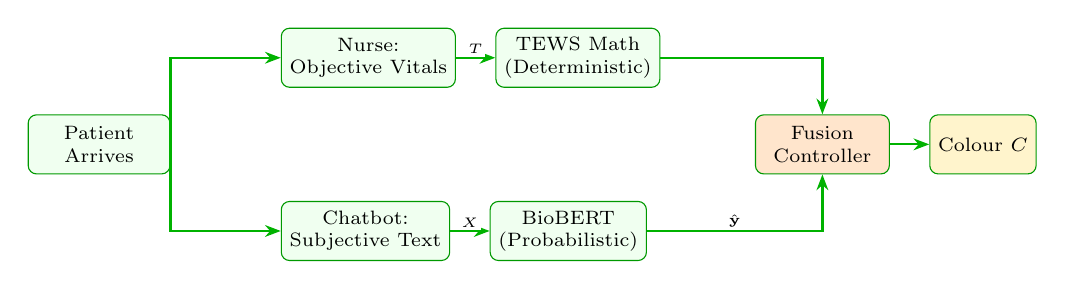
\begin{tikzpicture}[node distance=0.65cm and 0.5cm]
			\node[flowbox, minimum width=1.8cm] (patient) {Patient\\Arrives};
			\node[flowbox, right=1.4cm of patient, yshift=1.1cm] (nurse) {Nurse:\\Objective Vitals};
			\node[flowbox, right=of nurse] (tews) {TEWS Math\\(Deterministic)};
			\node[flowbox, right=1.4cm of patient, yshift=-1.1cm] (bot) {Chatbot:\\Subjective Text};
			\node[flowbox, right=of bot] (nlp) {BioBERT\\(Probabilistic)};
			\node[flowbox, right=1.2cm of tews, yshift=-1.1cm, fill=orange!20, minimum width=1.7cm] (fusion) {Fusion\\Controller};
			\node[flowbox, right=of fusion, fill=triageYellow!20, minimum width=1.3cm] (out) {Colour $C$};
			\draw[flowarr] (patient.east) |- (nurse.west);
			\draw[flowarr] (nurse) -- node[edgelabel, above] {$T$} (tews);
			\draw[flowarr] (tews.east) -| (fusion.north);
			\draw[flowarr] (patient.east) |- (bot.west);
			\draw[flowarr] (bot) -- node[edgelabel, above] {$X$} (nlp);
			\draw[flowarr] (nlp.east) -| node[edgelabel, pos=0.25, above] {$\hat{\mathbf{y}}$} (fusion.south);
			\draw[flowarr] (fusion) -- (out);
		\end{tikzpicture}}
	\end{center}
	\vspace{0.1cm}
	\small
	\begin{itemize}
		\item \textbf{TEWS:} Deterministic sum of vital-sign points from SATS tables: $T = \sum_k w_k f_k(v_k)$.
		\item \textbf{NLP:} Probabilistic classifier on chief-complaint text --- catches symptoms before vitals are measured.
		\item \textbf{Safety rule:} Fusion never assigns a less urgent colour than a strong language signal requires.
	\end{itemize}
\end{frame}

% =============================================================================
\section{NLP Pipeline}
% =============================================================================

\begin{frame}{NLP Analysis: Supervised Deep Learning}
	\begin{columns}[T]
		\begin{column}{0.58\textwidth}
			\begin{center}
				\resizebox{\textwidth}{!}{%
				
\begin{tikzpicture}[node distance=0.45cm and 0.35cm,
					pipe/.style={draw=green!60!black, rounded corners, fill=green!8,
						minimum height=0.65cm, minimum width=1.35cm, align=center, font=\tiny}]
					\node[pipe] (raw) {Chief\\Complaint};
					\node[pipe, right=of raw] (tok) {Tokenize};
					\node[pipe, right=of tok] (emb) {Embed\\768-d};
					\node[pipe, right=of emb] (bb) {BioBERT\\12 Layers};
					\node[pipe, right=of bb] (sm) {Softmax\\5 Classes};
					\node[pipe, right=of sm, fill=triageYellow!25] (sats) {SATS\\Colour};
					\foreach \a/\b in {raw/tok, tok/emb, emb/bb, bb/sm, sm/sats}
						\draw[flowarr] (\a) -- (\b);
				\end{tikzpicture}}
			\end{center}
			\vspace{0.15cm}
			\small
			\begin{itemize}
				\item \textbf{Supervised learning} on $\sim$80{,}000 nurse-labeled chief complaints.
				\item \textbf{Output:} Probabilities over 5 acuity levels $\to$ SATS colours (L1--2 Red/Orange; L3 Yellow; L4--5 Green).
				\item Bag-of-words fails: ``I do \textit{not} have a fever'' vs.\ ``I \textit{do} have a fever'' look identical to a word counter.
			\end{itemize}
		\end{column}
		\begin{column}{0.38\textwidth}
			\centering\scriptsize\textbf{Classification (Supervised)}
			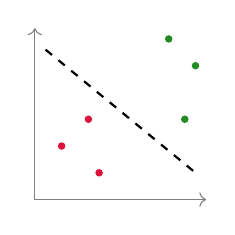
\begin{tikzpicture}[scale=0.68]
				\draw[->, gray] (0,0) -- (3.2,0);
				\draw[->, gray] (0,0) -- (0,3.2);
				\fill[triageRed] (0.5, 1) circle (2pt); \fill[triageRed] (1.2, 0.5) circle (2pt);
				\fill[triageRed] (1, 1.5) circle (2pt);
				\fill[triageGreen] (2.5, 3) circle (2pt); \fill[triageGreen] (3, 2.5) circle (2pt);
				\fill[triageGreen] (2.8, 1.5) circle (2pt);
				\draw[thick, dashed] (0.2, 2.8) -- (3, 0.5);
			\end{tikzpicture}
			\vspace{0.1cm}
			\footnotesize\textbf{Class imbalance:} Level 3 (Yellow) = 36\%; Level 1 (Red) = 4\%.
		\end{column}
	\end{columns}
\end{frame}

\begin{frame}{Tokenization: Raw Text to Integer IDs}
	\footnotesize
	Computers cannot read English --- they only understand numbers.
	$X \xrightarrow{\tau} (t_1, \ldots, t_M)$, $M \leq 128$.
	\begin{itemize}
		\item \textbf{WordPiece:} common words whole; rare words split (``headache'' $\to$ \texttt{head}+\texttt{\#\#ache})
		\item Vocabulary $\mathcal{V}$: $\sim$30{,}000 entries; each ID = row index in embedding table
	\end{itemize}
	\vspace{0.1cm}
	\centering
	\resizebox{0.92\textwidth}{!}{%
	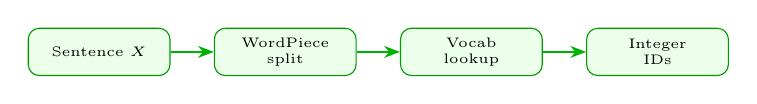
\begin{tikzpicture}[node distance=0.55cm,
		stepbox/.style={draw=green!60!black, rounded corners, fill=green!8,
			minimum height=0.6cm, minimum width=1.8cm, align=center, font=\tiny}]
		\node[stepbox] (sent) {Sentence $X$};
		\node[stepbox, right=of sent] (split) {WordPiece\\split};
		\node[stepbox, right=of split] (lookup) {Vocab\\lookup};
		\node[stepbox, right=of lookup] (ids) {Integer\\IDs};
		\foreach \a/\b in {sent/split, split/lookup, lookup/ids}
			\draw[flowarr] (\a) -- (\b);
	\end{tikzpicture}}
\end{frame}

\begin{frame}{Worked Example: Full ID Assignment}
	\scriptsize
	\textbf{Input:} ``I have a headache and feel feverish.'' \quad Each ID $\to$ row in $E_{\mathrm{word}}$.
	Real tokens: $M \approx 12$; batches pad to length 128 with filler tokens.
	\vspace{0.05cm}
	\begin{columns}[T]
		\begin{column}{0.48\textwidth}
			\begin{tabular}{@{}c l l c@{}}
				\toprule
				$i$ & Raw & Token & ID \\
				\midrule
				0 & --- & \texttt{[CLS]} & 101 \\
				1 & I & i & 1045 \\
				2 & have & have & 2031 \\
				3 & a & a & 1037 \\
				4 & headache & head+\#\#ache & 7994, 8772 \\
				5 & and & and & 1998 \\
				\bottomrule
			\end{tabular}
		\end{column}
		\begin{column}{0.48\textwidth}
			\begin{tabular}{@{}c l l c@{}}
				\toprule
				$i$ & Raw & Token & ID \\
				\midrule
				6 & feel & feel & 2514 \\
				7 & feverish & fever+\#\#ish & 9643, 6804 \\
				8 & . & . & 1012 \\
				9 & --- & \texttt{[SEP]} & 102 \\
				10 & --- & \texttt{[PAD]} & 0 \\
				11 & --- & \texttt{[PAD]} & 0 \\
				$\vdots$ & $\vdots$ & $\vdots$ & $\vdots$ \\
				127 & --- & \texttt{[PAD]} & 0 \\
				\bottomrule
			\end{tabular}
		\end{column}
	\end{columns}
	\vspace{0.06cm}
	\textbf{Vocabulary range:} token IDs $0 \ldots 28{,}995$ ($|\mathcal{V}| = 28{,}996$); sequence positions $i = 0 \ldots 127$ ($M \leq 128$).
	\vspace{0.04cm}
	\begin{tabular}{@{}l c p{7.4cm}@{}}
		\toprule
		\textbf{Special token} & \textbf{ID} & \textbf{Role} \\
		\midrule
		\texttt{[PAD]} & 0 & Padding filler after \texttt{[SEP]}; attention mask = 0 (ignored) \\
		\texttt{[UNK]} & 100 & Unknown WordPiece piece \\
		\texttt{[CLS]} & 101 & Classification summary (always $i=0$) \\
		\texttt{[SEP]} & 102 & Sentence boundary \\
		\texttt{[MASK]} & 103 & MLM pre-training only --- not used at triage inference \\
		\bottomrule
	\end{tabular}
\end{frame}

\begin{frame}{What is \texttt{[CLS]}?}
	\begin{columns}[T]
		\begin{column}{0.52\textwidth}
			\small
			\textbf{\texttt{[CLS]} = Classification token}
			\begin{itemize}
				\item Artificial token --- \textit{not} from the patient's words
				\item Always inserted at position $i = 0$ before any real text
				\item \textbf{Purpose:} After 12 transformer layers, its hidden state $h_{\mathrm{[CLS]}}$ becomes a 768-dimensional \textbf{summary} of the entire complaint
				\item This summary vector is multiplied by classification weights to predict acuity
			\end{itemize}
			\vspace{0.1cm}
			\texttt{[SEP]} (ID 102) marks the end of the sentence --- a boundary marker.
			\plain{Think of \texttt{[CLS]} as an empty notebook at the start. As the model reads every word, it fills that notebook with a compressed summary used for the final triage decision.}
		\end{column}
		\begin{column}{0.44\textwidth}
			\centering
			\resizebox{\textwidth}{!}{%
			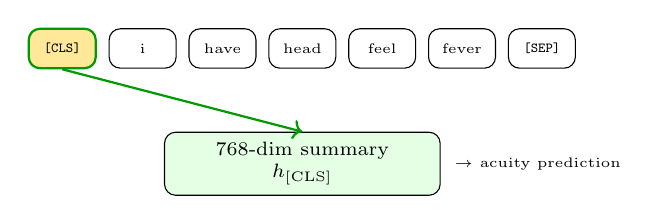
\begin{tikzpicture}[node distance=0.35cm,
				tok/.style={draw, rounded corners, minimum width=0.85cm, minimum height=0.5cm, font=\tiny, align=center},
				cls/.style={tok, fill=triageYellow!40, draw=green!60!black, thick}]
				\node[cls] (c) {\texttt{[CLS]}};
				\node[tok, right=0.15cm of c] (i) {i};
				\node[tok, right=0.15cm of i] (h) {have};
				\node[tok, right=0.15cm of h] (hd) {head};
				\node[tok, right=0.15cm of hd] (fe) {feel};
				\node[tok, right=0.15cm of fe] (fv) {fever};
				\node[tok, right=0.15cm of fv] (sep) {\texttt{[SEP]}};
				\node[draw, rounded corners, fill=green!10, minimum width=3.5cm, minimum height=0.8cm,
					below=0.8cm of hd, font=\scriptsize, align=center] (vec) {768-dim summary\\$h_{\mathrm{[CLS]}}$};
				\draw[->, thick, green!60!black] (c.south) -- (vec.north);
				\node[font=\tiny, right=0.05cm of vec] {$\to$ acuity prediction};
			\end{tikzpicture}}
		\end{column}
	\end{columns}
\end{frame}

\begin{frame}{Embedding Lookup: ID to 768-D Vector}
	\small
	A token ID alone carries no meaning. The \textbf{embedding layer} converts each ID to a dense vector:
	\[
		\mathbf{e}_i = E_{\mathrm{word}}[\mathrm{id}(t_i)] \in \mathbb{R}^{768}
	\]
	\begin{columns}[T]
		\begin{column}{0.46\textwidth}
			\textbf{Variables:}
			\begin{itemize}
				\item $V \approx 30{,}000$ --- vocabulary size (rows)
				\item $D = 768$ --- embedding dimension (columns)
				\item $E_{\mathrm{word}} \in \mathbb{R}^{V \times 768}$ --- learned weight matrix
				\item ID 2031 $\to$ row 2031 $\to$ vector $[0.04, -0.21, \ldots, 0.17]$
			\end{itemize}
			\plain{The embedding table is like a dictionary where each word ID points to a list of 768 numbers that encode its meaning.}
		\end{column}
		\begin{column}{0.50\textwidth}
			\centering
			\resizebox{\textwidth}{!}{%
			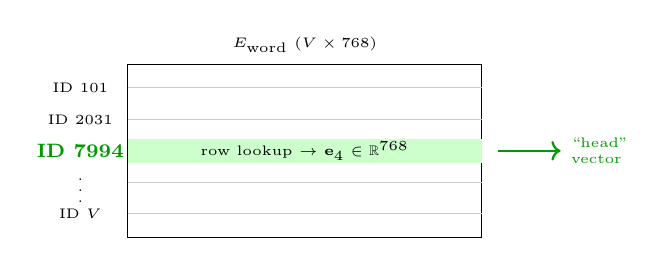
\begin{tikzpicture}[font=\tiny]
				\draw (0,0) rectangle (4.5,2.2);
				\node at (2.25,2.45) {$E_{\mathrm{word}}$ ($V \times 768$)};
				\foreach \y in {0.3,0.7,1.1,1.5,1.9} {
					\draw[gray!40] (0,\y) -- (4.5,\y);
				}
				\node at (-0.6,1.9) {ID 101};
				\node at (-0.6,1.5) {ID 2031};
				\node[font=\scriptsize\bfseries, green!60!black] at (-0.6,1.1) {ID 7994};
				\node at (-0.6,0.7) {$\vdots$};
				\node at (-0.6,0.3) {ID $V$};
				\fill[green!20] (0,0.95) rectangle (4.5,1.25);
				\node at (2.25,1.1) {row lookup $\to$ $\mathbf{e}_4 \in \mathbb{R}^{768}$};
				\draw[->, thick, green!60!black] (4.7,1.1) -- (5.5,1.1)
					node[right, align=left] {``head''\\vector};
			\end{tikzpicture}}
		\end{column}
	\end{columns}
\end{frame}

\begin{frame}{What the Vector Represents}
	\begin{columns}[T]
		\begin{column}{0.48\textwidth}
			\small
			Each of the 768 dimensions is a \textbf{learned feature} --- not hand-designed.
			\begin{itemize}
				\item Similar words have similar vectors (close in space)
				\item ``headache'', ``feverish'', ``aches'' cluster near ``pain'', ``fever'' in BioBERT's PubMed-trained space
				\item \textbf{Static} (Word2Vec): one vector per word forever
				\item \textbf{Contextual} (BERT): same word, different vector depending on sentence --- next slide
			\end{itemize}
			\vspace{0.1cm}
			Example vector for ``headache'':\\
			$\mathbf{e} = [0.12,\,-0.45,\,0.88,\,\ldots,\,-0.01]$ (768 numbers)
		\end{column}
		\begin{column}{0.48\textwidth}
			\begin{center}
				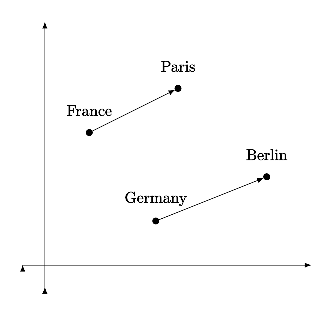
\includegraphics[height=0.36\textheight, keepaspectratio]{assets/word_embedding.pdf}
			\end{center}
			\footnotesize Word vectors in semantic space.\footnote{Word embedding illustration, Fschwarzentruber, Wikimedia Commons.}
		\end{column}
	\end{columns}
\end{frame}

\begin{frame}{Contextual Mapping: Three Embeddings Summed}
	\begin{center}
		\resizebox{0.88\textwidth}{!}{%
		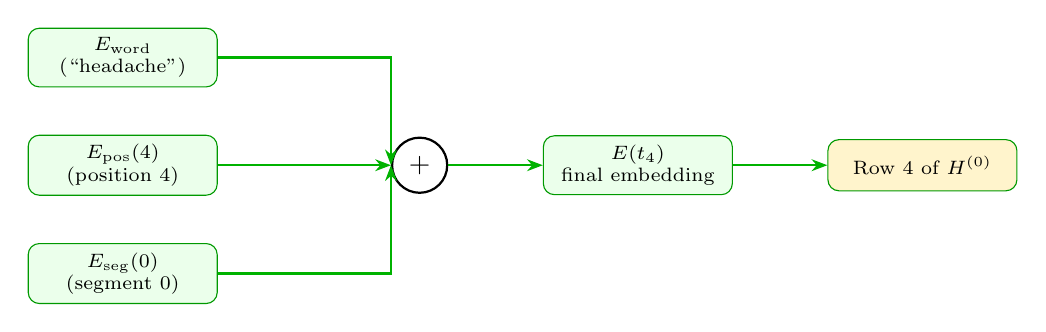
\begin{tikzpicture}[node distance=0.6cm and 1.2cm,
			emb/.style={draw=green!60!black, rounded corners, fill=green!8,
				minimum width=2.4cm, minimum height=0.65cm, align=center, font=\scriptsize}]
			\node[emb] (ew) {$E_{\mathrm{word}}$\\(``headache'')};
			\node[emb, below=of ew] (ep) {$E_{\mathrm{pos}}(4)$\\(position 4)};
			\node[emb, below=of ep] (es) {$E_{\mathrm{seg}}(0)$\\(segment 0)};
			\node[circle, draw, thick, minimum size=0.7cm, right=2.2cm of ep] (plus) {$+$};
			\node[emb, right=1.2cm of plus] (ef) {$E(t_4)$\\final embedding};
			\node[emb, right=1.2cm of ef, fill=triageYellow!20] (row) {Row 4 of $H^{(0)}$};
			\draw[flowarr] (ew.east) -| (plus.west);
			\draw[flowarr] (ep) -- (plus);
			\draw[flowarr] (es.east) -| (plus.west);
			\draw[flowarr] (plus) -- (ef);
			\draw[flowarr] (ef) -- (row);
		\end{tikzpicture}}
	\end{center}
	\vspace{0.1cm}
	\small Three separate learned vectors are \textbf{added element-wise} for each token position $i$ to produce the input embedding $E(t_i)$.
\end{frame}

\begin{frame}{Contextual Mapping: Formula Breakdown}
	\small
	\[
		E(t_i) = E_{\mathrm{word}}(t_i) + E_{\mathrm{pos}}(i) + E_{\mathrm{seg}}(t_i)
	\]
	\begin{tabular}{@{}p{2.2cm}p{4.5cm}p{4.5cm}@{}}
		\toprule
		\textbf{Term} & \textbf{Meaning} & \textbf{Example} \\
		\midrule
		$E_{\mathrm{word}}$ & Token identity --- what word is this? & ``headache'' vs ``feverish'' \\
		$E_{\mathrm{pos}}(i)$ & Position in sentence --- order matters & ``head ache'' $\neq$ ``ache head'' \\
		$E_{\mathrm{seg}}$ & Which sentence (A or B) & 0 for our single complaint \\
		\bottomrule
	\end{tabular}

	\vspace{0.1cm}
	\textbf{Bidirectional reading:} BERT sees all tokens left \textit{and} right --- ``feel feverish'' informs ``headache'' in both directions.

	\footnotesize\textit{The word ``feel'' at position 6 gets a different $E_{\mathrm{pos}}$ than at position 12 in a longer sentence.}
\end{frame}

\begin{frame}{The Input Matrix $H^{(0)}$}
	\small
	After embedding every token, the full sentence becomes a matrix:
	\[
		H^{(0)} \in \mathbb{R}^{M \times 768}
	\]
	Each \textbf{row} = one token's 768-dimensional embedding. Each \textbf{column} = one feature dimension across all tokens.

	\vspace{0.15cm}
	\centering
	\resizebox{0.92\textwidth}{!}{%
	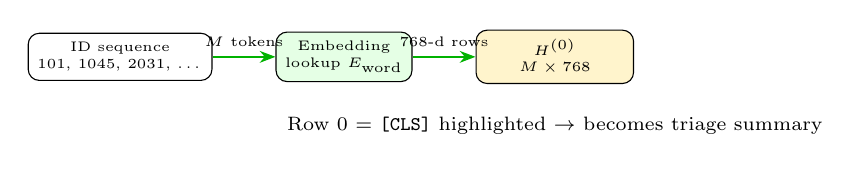
\begin{tikzpicture}[node distance=0.5cm,
		box/.style={draw, rounded corners, minimum height=0.55cm, minimum width=1.4cm, align=center, font=\tiny}]
		\node[box] (ids) {ID sequence\\101, 1045, 2031, \ldots};
		\node[box, right=0.8cm of ids, fill=green!10] (lookup) {Embedding\\lookup $E_{\mathrm{word}}$};
		\node[box, right=0.8cm of lookup, fill=triageYellow!20, minimum width=2cm] (mat) {$H^{(0)}$\\$M \times 768$};
		\draw[flowarr] (ids) -- node[above, font=\tiny] {$M$ tokens} (lookup);
		\draw[flowarr] (lookup) -- node[above, font=\tiny] {768-d rows} (mat);
		\node[below=0.3cm of mat, font=\scriptsize, align=center] {Row 0 = \texttt{[CLS]} highlighted $\to$ becomes triage summary};
	\end{tikzpicture}}

	\vspace{0.1cm}
	\footnotesize The matrix shape stays $M \times 768$ through all 12 layers --- only the \textit{values} inside change.
\end{frame}

\begin{frame}{Matrix Walkthrough with Numbers}
	\footnotesize
	\textbf{Example submatrix} (first 4 of 768 dimensions shown):
	\begin{tabular}{|c|l|c|c|c|c|c|}
		\hline
		\textbf{$i$} & \textbf{Token} & $D_1$ & $D_2$ & $D_3$ & $D_4$ & $\cdots$ \\
		\hline
		0 & \texttt{[CLS]} & $0.02$ & $0.11$ & $-0.05$ & $0.33$ & $\cdots$ \\
		\hline
		1 & i & $-0.08$ & $0.04$ & $0.19$ & $0.01$ & $\cdots$ \\
		\hline
		2 & have & $0.15$ & $-0.22$ & $0.07$ & $0.44$ & $\cdots$ \\
		\hline
		4 & head & $0.31$ & $-0.18$ & $0.52$ & $0.09$ & $\cdots$ \\
		\hline
		7 & fever & $0.44$ & $0.27$ & $-0.11$ & $0.61$ & $\cdots$ \\
		\hline
		$\vdots$ & $\vdots$ & $\vdots$ & $\vdots$ & $\vdots$ & $\vdots$ & $\vdots$ \\
		\hline
	\end{tabular}

	\vspace{0.15cm}
	\small
	After $L=12$ transformer layers: $h_{\mathrm{[CLS]}} = H^{(12)}_{0,:}$ --- the first row of the final layer output, a single 768-dim vector summarising the complaint.
\end{frame}

\begin{frame}{Diagram: 12 Stacked Encoder Layers}
	\begin{center}
		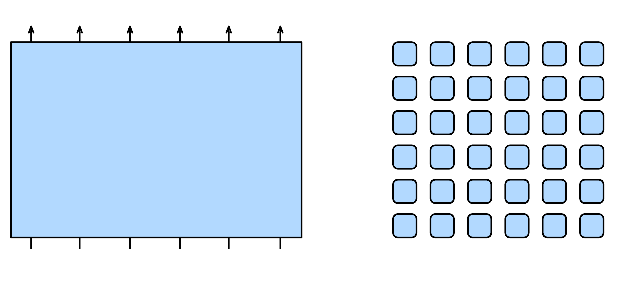
\includegraphics[height=0.72\textheight, keepaspectratio]{assets/bert_encoder.pdf}
	\end{center}
	\footnotesize Diagram: Zhang et al., d2l-ai, CC BY-SA 4.0. Each block = one encoder layer (self-attention + feed-forward).
\end{frame}

\begin{frame}{Inside One Encoder Layer: Formulas}
	\small
	Each layer $\ell = 1, \ldots, 12$ performs two sub-steps with \textbf{residual connections}:
	\begin{align*}
		Z^{(\ell)} &= \mathrm{LayerNorm}\!\bigl(H^{(\ell-1)} + \mathrm{MultiHeadAttention}(H^{(\ell-1)})\bigr) \\
		H^{(\ell)} &= \mathrm{LayerNorm}\!\bigl(Z^{(\ell)} + \mathrm{FFN}(Z^{(\ell)})\bigr)
	\end{align*}
	\begin{tabular}{@{}p{3.2cm}p{8.5cm}@{}}
		\toprule
		\textbf{Component} & \textbf{What it does} \\
		\midrule
		MultiHeadAttention & 12 parallel self-attention heads; each learns different word relationships \\
		FFN & Two linear layers: $\mathrm{FFN}(x) = W_2\,\mathrm{ReLU}(W_1 x + b_1) + b_2$ \\
		LayerNorm & Normalises activations --- stabilises training across 12 layers \\
		Residual ($+$) & Adds input back to output --- prevents information loss in deep stacks \\
		\bottomrule
	\end{tabular}
\end{frame}

\begin{frame}{Stacking 12 Layers: From Words to Clinical Understanding}
	\small
	\[
		H^{(0)} \xrightarrow{\text{Layer 1}} H^{(1)} \xrightarrow{\text{Layer 2}} \cdots \xrightarrow{\text{Layer 12}} H^{(12)} = H^{(L)}
	\]
	\begin{itemize}
		\item \textbf{Shallow layers} (1--4): recognise individual words and simple phrases
		\item \textbf{Middle layers} (5--8): combine symptoms --- ``headache'' + ``feverish'' + ``weak''
		\item \textbf{Deep layers} (9--12): abstract clinical urgency patterns
		\item \textbf{Parallel processing:} all $M$ tokens processed simultaneously (not left-to-right)
	\end{itemize}
	\vspace{0.15cm}
	\textbf{Output:} $h_{\mathrm{[CLS]}} = H^{(L)}_{0,:} \in \mathbb{R}^{768}$ $\to$ fed to the classification head.
	\plain{Stacking layers is like reading a complaint once for words, once for phrases, and once for overall urgency.}
\end{frame}

\begin{frame}{Self-Attention Mechanism}
	\begin{center}
		\resizebox{!}{0.78\textheight}{%
		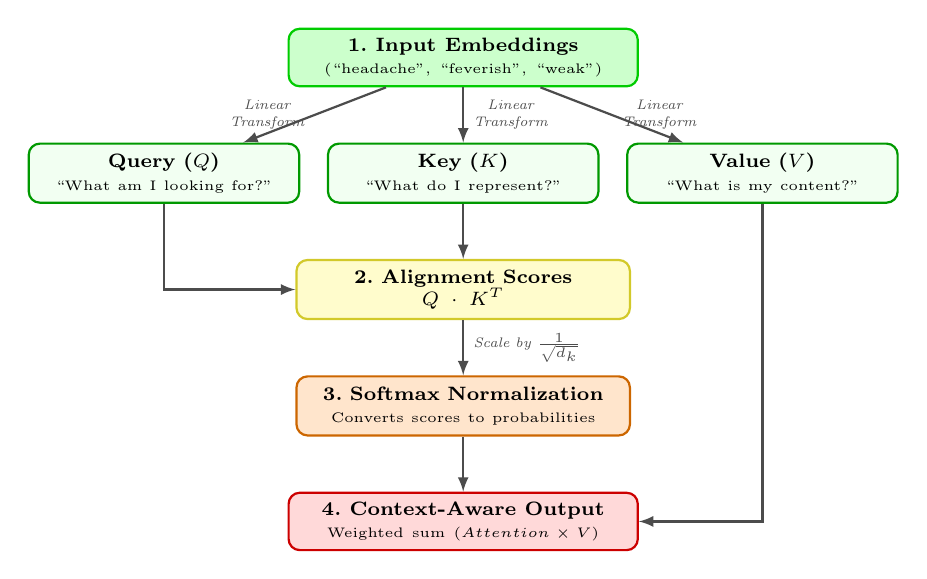
\begin{tikzpicture}[node distance=0.7cm, thick,
			box/.style={draw=green!60!black, rectangle, fill=green!5, text width=3.2cm, align=center, minimum height=0.75cm, rounded corners, font=\scriptsize},
			highlightbox/.style={draw=green!80!black, rectangle, fill=green!20, text width=4.2cm, align=center, minimum height=0.7cm, rounded corners, font=\scriptsize\bfseries},
			arrow/.style={->, >=latex, thick, draw=black!70},
			label/.style={font=\tiny\itshape, text=black!70, align=center}
			]
			\node[highlightbox] (input) {1.\ Input Embeddings\\ \mdseries \tiny (``headache'', ``feverish'', ``weak'')};
			\node[box, below=0.7cm of input, xshift=-3.8cm] (query) {\textbf{Query ($Q$)}\\ \tiny ``What am I looking for?''};
			\node[box, below=0.7cm of input] (key) {\textbf{Key ($K$)}\\ \tiny ``What do I represent?''};
			\node[box, below=0.7cm of input, xshift=3.8cm] (value) {\textbf{Value ($V$)}\\ \tiny ``What is my content?''};
			\node[box, fill=yellow!20, draw=yellow!80!black, below=0.7cm of key, text width=4cm] (matmul) {\textbf{2.\ Alignment Scores}\\ $Q \cdot K^T$};
			\node[box, fill=orange!20, draw=orange!80!black, below=0.7cm of matmul, text width=4cm] (softmax) {\textbf{3.\ Softmax Normalization}\\ \mdseries \tiny Converts scores to probabilities};
			\node[highlightbox, fill=red!15, draw=red!80!black, below=0.7cm of softmax, text width=4.2cm] (output) {\textbf{4.\ Context-Aware Output}\\ \mdseries \tiny Weighted sum ($Attention \times V$)};
			\draw[arrow] (input) -- node[label, left] {Linear\\Transform} (query);
			\draw[arrow] (input) -- node[label, right] {Linear\\Transform} (key);
			\draw[arrow] (input) -- node[label, right] {Linear\\Transform} (value);
			\draw[arrow] (query) |- (matmul);
			\draw[arrow] (key) -- (matmul);
			\draw[arrow] (matmul) -- node[label, right] {Scale by $\frac{1}{\sqrt{d_k}}$} (softmax);
			\draw[arrow] (softmax) -- (output);
			\draw[arrow] (value) |- (output);
		\end{tikzpicture}}
	\end{center}
\end{frame}

\begin{frame}{Self-Attention Equation: Variable by Variable}
	\small
	From Vaswani et al.\ (2017):
	\[
		\mathrm{Attention}(Q,K,V) = \mathrm{softmax}\!\left(\frac{QK^{\top}}{\sqrt{d_k}}\right)V
	\]
	\begin{tabular}{@{}p{1.5cm}p{4.5cm}p{4.8cm}@{}}
		\toprule
		\textbf{Symbol} & \textbf{Definition} & \textbf{Role in triage} \\
		\midrule
		$Q$ & Query matrix $= H W_Q$ & ``What is this token looking for?'' \\
		$K$ & Key matrix $= H W_K$ & ``What does each token offer?'' \\
		$V$ & Value matrix $= H W_V$ & Semantic content passed forward \\
		$d_k$ & Key dimension ($= 64$ per head) & Scaling factor \\
		$QK^\top$ & Pairwise relevance scores & ``headache'' $\leftrightarrow$ ``feverish'' co-attend \\
		$\sqrt{d_k}$ & Prevents dot products exploding & Training stability \\
		\bottomrule
	\end{tabular}

	\vspace{0.1cm}
	\footnotesize\textbf{Worked weights} for query ``headache'': feverish 0.41, headache 0.32, weak 0.18, filler words $\approx 0.02$.
\end{frame}

% =============================================================================
\section{BERT Pre-Training}
% =============================================================================

\begin{frame}{BERT Pre-Training: Masked Language Modeling}
	\small
	Before triage fine-tuning, BioBERT learns medical English from PubMed via \textbf{Masked Language Modeling (MLM)}:
	\begin{center}
		\resizebox{0.88\textwidth}{!}{%
		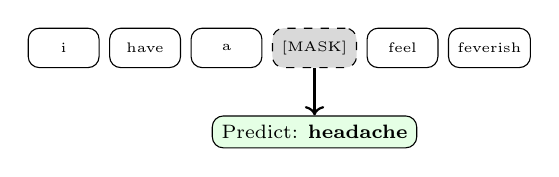
\begin{tikzpicture}[node distance=0.35cm,
			tok/.style={draw, rounded corners, minimum width=0.9cm, minimum height=0.5cm, font=\tiny, align=center},
			mask/.style={tok, fill=gray!30, dashed}]
			\node[tok] (i) {i};
			\node[tok, right=0.12cm of i] (h) {have};
			\node[tok, right=0.12cm of h] (a) {a};
			\node[mask, right=0.12cm of a] (m) {[MASK]};
			\node[tok, right=0.12cm of m] (f) {feel};
			\node[tok, right=0.12cm of f] (fv) {feverish};
			\node[draw, rounded corners, fill=green!10, below=0.6cm of m, font=\scriptsize] (pred) {Predict: \textbf{headache}};
			\draw[->, thick] (m) -- (pred);
		\end{tikzpicture}}
	\end{center}
	\begin{itemize}
		\item 15\% of tokens randomly masked; model predicts them from \textbf{bidirectional} context
		\item Teaches medical vocabulary (``feverish'', ``headache'', ``tachycardia'') before any triage labels
		\item BioBERT = BERT pre-trained on PubMed + PMC biomedical abstracts
	\end{itemize}
\end{frame}

\begin{frame}{MLM Loss Formula}
	\small
	\begin{block}{Masked Language Modeling Loss}
		\[
			\mathcal{L}_{\mathrm{LM}} = -\sum_{i \in \mathcal{M}} \log P(t_i \mid H^{(L)};\, \theta)
		\]
	\end{block}
	\begin{tabular}{@{}p{2.5cm}p{8.5cm}@{}}
		\toprule
		\textbf{Variable} & \textbf{Meaning} \\
		\midrule
		$\mathcal{M}$ & Set of masked token positions in the sentence \\
		$t_i$ & The true (correct) word at masked position $i$ \\
		$H^{(L)}$ & Final hidden states from all 12 layers --- the context \\
		$\theta$ & All model parameters (weights + biases) \\
		$P(t_i \mid \cdot)$ & Softmax probability the model assigns to the correct word \\
		$\mathcal{L}_{\mathrm{LM}}$ & Total penalty --- lower = better word predictions \\
		\bottomrule
	\end{tabular}
\end{frame}

\begin{frame}{Independent vs.\ Dependent Variables in MLM}
	\small
	\begin{itemize}
		\item \textbf{Independent variable ($H^{(L)}$):} The surrounding, unmasked context the model is allowed to read bidirectionally
		\item \textbf{Dependent variable ($\mathcal{L}_{\mathrm{LM}}$):} The loss penalty --- its size depends entirely on $P(t_i)$ the model assigned to the correct hidden word
	\end{itemize}
	\vspace{0.15cm}
	\textbf{Numerical example:}
	\begin{itemize}
		\item Correct word = ``headache''; model assigns $P = 0.92$ $\Rightarrow$ contribution $= -\log(0.92) \approx 0.08$ (small penalty)
		\item Model assigns $P = 0.01$ to correct word $\Rightarrow$ $-\log(0.01) \approx 4.6$ (large penalty)
	\end{itemize}
	\vspace{0.1cm}
	\plain{After MLM pre-training on PubMed, BioBERT is fine-tuned on 80{,}000 triage-labeled chief complaints using cross-entropy loss --- covered next.}
\end{frame}

% =============================================================================
\section{Learning Math}
% =============================================================================

\begin{frame}{Attention Softmax: The Probability Filter}
	\small
	To assign mathematical weight to each word, raw scores are normalised:
	\[
		\alpha_j = \frac{\exp(e_j)}{\sum_{k=1}^{m}\exp(e_k)}
	\]
	\begin{tabular}{@{}p{2.5cm}p{8.5cm}@{}}
		\toprule
		\textbf{Variable} & \textbf{Meaning} \\
		\midrule
		$e_j$ & Raw attention score for token $j$ (before normalisation) \\
		$\exp(e_j)$ & Forces positive values; amplifies large scores \\
		$\sum_k \exp(e_k)$ & Normalising constant --- ensures all weights sum to 1 \\
		$\alpha_j$ & Final attention weight for token $j$ (a probability) \\
		$m$ & Sequence length (number of tokens) \\
		\bottomrule
	\end{tabular}

	\vspace{0.1cm}
	\textbf{Effect:} ``I'', ``a'', ``and'' $\to$ $\alpha \approx 0.01$; ``headache'', ``feverish'' $\to$ $\alpha \approx 0.35+$.
\end{frame}

\begin{frame}{Classification Softmax: Acuity Probabilities}
	\small
	The summary vector is mapped to triage class probabilities:
	\[
		\hat{\mathbf{y}} = \mathrm{softmax}(W h_{\mathrm{[CLS]}} + \mathbf{b}), \quad \hat{y}_c = P(\text{acuity} = c \mid X)
	\]
	\begin{tabular}{@{}p{2.8cm}p{8.2cm}@{}}
		\toprule
		\textbf{Variable} & \textbf{Meaning} \\
		\midrule
		$h_{\mathrm{[CLS]}}$ & 768-dim summary vector from final layer \\
		$W \in \mathbb{R}^{5 \times 768}$ & Learned classification weight matrix \\
		$\mathbf{b} \in \mathbb{R}^{5}$ & Per-class bias terms \\
		$\hat{y}_c$ & Probability of acuity level $c \in \{1,\ldots,5\}$ \\
		$\sum_c \hat{y}_c = 1$ & Valid probability distribution over 5 classes \\
		\bottomrule
	\end{tabular}

	\vspace{0.1cm}
	\begin{exampleblock}{Worked example --- our running complaint}
		\footnotesize
		\complaint\\
		Level 3 (Moderate): \textbf{72\%} $\Rightarrow$ maps to \textcolor{triageYellow}{\textbf{Yellow}}
	\end{exampleblock}
\end{frame}

\begin{frame}{Forward Pass and Cross-Entropy Loss}
	\small
	\begin{block}{1. Forward Pass}
		$y = Wx + b$ \quad where $x = h_{\mathrm{[CLS]}}$, $y$ = predicted logits, $W$ and $b$ are learned.
	\end{block}
	\begin{block}{2. Cross-Entropy Loss (The Penalty)}
		$\mathcal{L} = -\sum_{i=1}^{C} y_i \log(\hat{y}_i)$ \quad where $C = 5$ acuity classes.
	\end{block}
	\begin{tabular}{@{}p{1.8cm}p{9.2cm}@{}}
		\toprule
		\textbf{Symbol} & \textbf{Meaning} \\
		\midrule
		$x$ & Input vector ($h_{\mathrm{[CLS]}}$ --- the complaint summary) \\
		$W, b$ & Weights and bias the model must learn \\
		$y$ & True one-hot nurse label (e.g.\ Level 3 = Yellow) \\
		$\hat{y}$ & Model's predicted probability distribution \\
		$\mathcal{L}$ & Loss --- 0 if perfect; large if wrong with high confidence \\
		\bottomrule
	\end{tabular}

	\vspace{0.1cm}
	\footnotesize Example: true label = Yellow, model predicts Green at 90\% $\Rightarrow$ $\mathcal{L} = -\log(0.05) \approx 3.0$.
\end{frame}

\begin{frame}{Backpropagation: The Chain Rule}
	\small
	\begin{block}{3. Backpropagation (The Investigation)}
		\[
			\frac{\partial \mathcal{L}}{\partial W} = \frac{\partial \mathcal{L}}{\partial \hat{y}} \cdot \frac{\partial \hat{y}}{\partial z} \cdot \frac{\partial z}{\partial W}
		\]
	\end{block}
	\begin{itemize}
		\item Uses the \textbf{chain rule} of calculus to travel backward through all 12 layers + classification head
		\item $z = Wh + b$ --- pre-softmax logits (raw scores before probability conversion)
		\item Each partial derivative pinpoints which specific weight caused the bad guess
		\item Gradients flow from the loss at the top back to every embedding and attention weight
	\end{itemize}
	\plain{If the model confidently assigns 90\% to Green when the nurse labeled Yellow, backprop finds exactly which weights in layers 8--12 over-weighted non-urgent patterns.}
\end{frame}

\begin{frame}{Gradient Descent and Fine-Tuning}
	\small
	\begin{block}{4. Optimization (The Correction)}
		\[
			W_{\mathrm{new}} = W_{\mathrm{old}} - \alpha \frac{\partial \mathcal{L}}{\partial W}
		\]
	\end{block}
	\begin{tabular}{@{}p{2.5cm}p{8.5cm}@{}}
		\toprule
		\textbf{Variable} & \textbf{Meaning} \\
		\midrule
		$\alpha$ & Learning rate (step size; e.g.\ $2 \times 10^{-5}$) \\
		$\partial \mathcal{L}/\partial W$ & Gradient --- direction of steepest loss \textit{increase} \\
		Minus sign ($-$) & Move \textit{opposite} to gradient --- go downhill on the loss surface \\
		\bottomrule
	\end{tabular}

	\vspace{0.15cm}
	\textbf{Fine-tuning loss} on triage data:
	\[
		\mathcal{L}_{\mathrm{triage}} = -\sum_{i=1}^{N} \log P(y_i \mid X_i;\, \theta), \quad N \approx 80{,}000
	\]
	\footnotesize Best eval\_loss $= 0.001812$ after 3 epochs (13{,}500 steps) on nurse-labeled chief complaints.
\end{frame}

% =============================================================================
\section{Summary}
% =============================================================================

\begin{frame}{End-to-End: Complaint to Triage Colour}
	\begin{columns}[T]
		\begin{column}{0.52\textwidth}
			\small
			\textbf{Putting it all together} for our running example:
			\begin{enumerate}
				\item Patient says: \complaint
				\item Tokenize $\to$ embed $\to$ 12 transformer layers
				\item Self-attention weights ``headache'', ``feverish'', ``weak'' heavily
				\item $h_{\mathrm{[CLS]}} \to$ softmax $\to$ Level 3 at 72\%
				\item Fusion with TEWS vitals $\to$ final \textcolor{triageYellow}{\textbf{Yellow}} pathway
			\end{enumerate}
			\vspace{0.1cm}
			\footnotesize Trained on $\sim$80{,}000 nurse-labeled complaints; BioBERT pre-trained on PubMed MLM.
		\end{column}
		\begin{column}{0.44\textwidth}
			\begin{center}
				\resizebox{!}{0.62\textheight}{%
				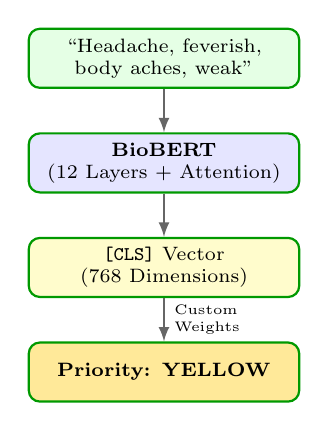
\begin{tikzpicture}[node distance=0.55cm, auto, thick,
					box/.style={draw=green!60!black, rectangle, fill=green!10, text width=3.2cm, align=center, minimum height=0.75cm, rounded corners, font=\scriptsize},
					arrow/.style={->, >=latex, thick, draw=black!60}]
					\node[box] (input) {``Headache, feverish,\\body aches, weak''};
					\node[box, fill=blue!10, below=of input] (biobert) {\textbf{BioBERT}\\ (12 Layers + Attention)};
					\node[box, fill=yellow!20, below=of biobert] (vector) {\texttt{[CLS]} Vector\\(768 Dimensions)};
					\node[box, fill=triageYellow!40, below=of vector] (output) {\textbf{Priority: YELLOW}};
					\draw[arrow] (input) -- (biobert);
					\draw[arrow] (biobert) -- (vector);
					\draw[arrow] (vector) -- node[right, font=\tiny, text width=1.2cm, align=left] {Custom\\Weights} (output);
				\end{tikzpicture}}
			\end{center}
		\end{column}
	\end{columns}
\end{frame}

\end{document}
